\documentclass[10pt]{article}

%---------------------------------------------------------------------
\usepackage[a4paper, headsep=-4in,bindingoffset=0in,%
left=2.5cm,right=2.5cm,top=2.5cm,bottom=2.5cm,%
footskip=.25in]{geometry}

%\usepackage[english]{babel}   
\usepackage[utf8]{inputenc}  
\usepackage{tgbonum}
\usepackage[font=scriptsize]{caption}

%\DeclareCaptionFont{6pt}{\fontsize{6pt}{6pt}\selectfont}
\captionsetup[figure]{font={stretch=1}}  
%\usepackage{sectsty}
\usepackage{subcaption}
\usepackage{wrapfig}
\usepackage{layout}
\usepackage{graphicx}
\usepackage{verbatim}
\usepackage{listings}
\usepackage{mathptmx}
\usepackage[backend=biber,style=apa,sorting=none]{biblatex}
\addbibresource{paperpile.bib}
%\pagenumbering{gobble}
\pagenumbering{arabic}

\usepackage{amsfonts}
\graphicspath{{figs/}}
\setlength{\topmargin}{-10pt}
%\renewcommand{\baselinestretch}{1.5}

\usepackage{indentfirst}
\setlength{\parindent}{1cm}

\setlength{\headsep}{1pt}
%---------------------------------------------------------------------

\begin{document} 

{\large \section*{}}
\begin{center}
Emily Olafson$^1*$, Keith Jamison$^1$, Amy Kuceyeski$^1$
\end{center}

    1. \textmd{Department of Radiology, Weill Cornell Medical College, New York City, New York, USA, 10021} 

%---------------------------------------------------------------------

\section{Introduction}
Ischemic stroke is a leading cause of physical impairment worldwide. Up to one-third of stroke survivors have poor motor outcomes five years after stroke, but the ability to predict long-term deficits from acute clinical information is still a major challenge.

The location of the stroke in the brain explains some of the variance in long-term outcomes, but it is currently unclear how to best extract information from lesion data for predictive models (\cite{Sperber2020-kp, Kasties2021-rm}). The most widely-employed lesion biomarker of motor outcome is the corticospinal tract (CST) lesion load, or the proportion of voxels in the ipsilesional corticospinal tract (typically consisting of fibers from primary motor cortex) that intersect with the lesion (\cite{Zhu2010-qh, Feng2015-du}). This biomarker has been related to motor deficits in the acute phase of stroke, but it is unclear whether this biomarker can accurately predict chronic impairments across a wide range of lesion topographies (for review, see \cite{Kim2017-xe}). 
Models that incorporate information about how the lesion damages additional sensorimotor regions, i.e. regions beyond the primary motor cortex that are still related to motor and sensory function, explain more variance in post-stroke outcome compared to models that incorporate information about primary motor cortex CST damage alone (\cite{Ito2022-em, Sperber2021-lw, Rondina2016-ds, Rondina2017-ij, Schulz2012-yy}). These more complex models tend to incorporate damage to premotor, supplementary motor, pre-supplementary motor, and somatosensory cortices (\cite{Ito2022-em,Schulz2012-yy, Sperber2021-lw}) as well as the extent of overlap between the lesion and subcortical regions like the thalamus and basal ganglia (\cite{Rondina2016-ds, Rondina2017-ij}). 


Recently, \cite{Bowren2022-rs} have attempted to use maps derived from lesion-network mapping to predict motor outcomes, with the idea that the structural connections that are most strongly associated with chronic motor outcomes in one dataset may be useful for predicting chronic outcomes in an independent dataset. They generated lesion-network maps that reflect the structural connectivity seeded from the voxels where there is the strongest association between lesion damage and motor deficits. The extent of overlap between a lesion and this map, called the structural lesion-network map lesion load, was related to motor scores.   

Although predictions of chronic motor outcome are made more accurate by incorporating measures of damage to sensorimotor regions, the optimal set of features extracted from lesion data may not be directly related to hemiparesis per se (\cite{Bzdok2020-py, Sperber2021-lw}). Because of the hierarchical, non-random distribution of lesion topography (\cite{Mah2014-cb,Wang2019-dz}), damage to voxels outside of the motor system may meaningfully predict chronic motor impairment (\cite{Sperber2021-lw}). Machine learning models that incorporate features in a data-driven way may be able to discover lesion-deficit associations that are useful in predictions beyond the current suite of theory-driven biomarkers like those in the motor system (\cite{Kasties2021-rm, Calesella2021-kp}).





In this paper, we compare the predictive accuracy of several imaging biomarkers of post-stroke motor impairment and rigorously assess their out-of-sample performance using the ENIGMA dataset, a multi-site stroke lesion database (\cite{Liew2020-ps}).
Crucially, most biomarkers explored to date have not been tested on independent data using cross-validation (\cite{Kim2017-xe}), despite using machine learning methods that are prone to overfitting in high-dimensional settings (\cite{Hastie2001-or}). 




\section{Materials and methods}


\subsection{Model specification}

\subsubsection{Lesion load of primary motor cortex}
The M1-corticospinal tract segmentation was obtained from the sensorimotor area tract template (SMATT) (\cite{Archer2018-ti}). M1-CST lesion load was calculated as the proportion of lesioned voxels intersecting with the ipsilesional M1-CST (\cite{Zhu2010-qh}).


\subsubsection{Lesion load beyond M1}
\begin{figure}[htp]
\centering
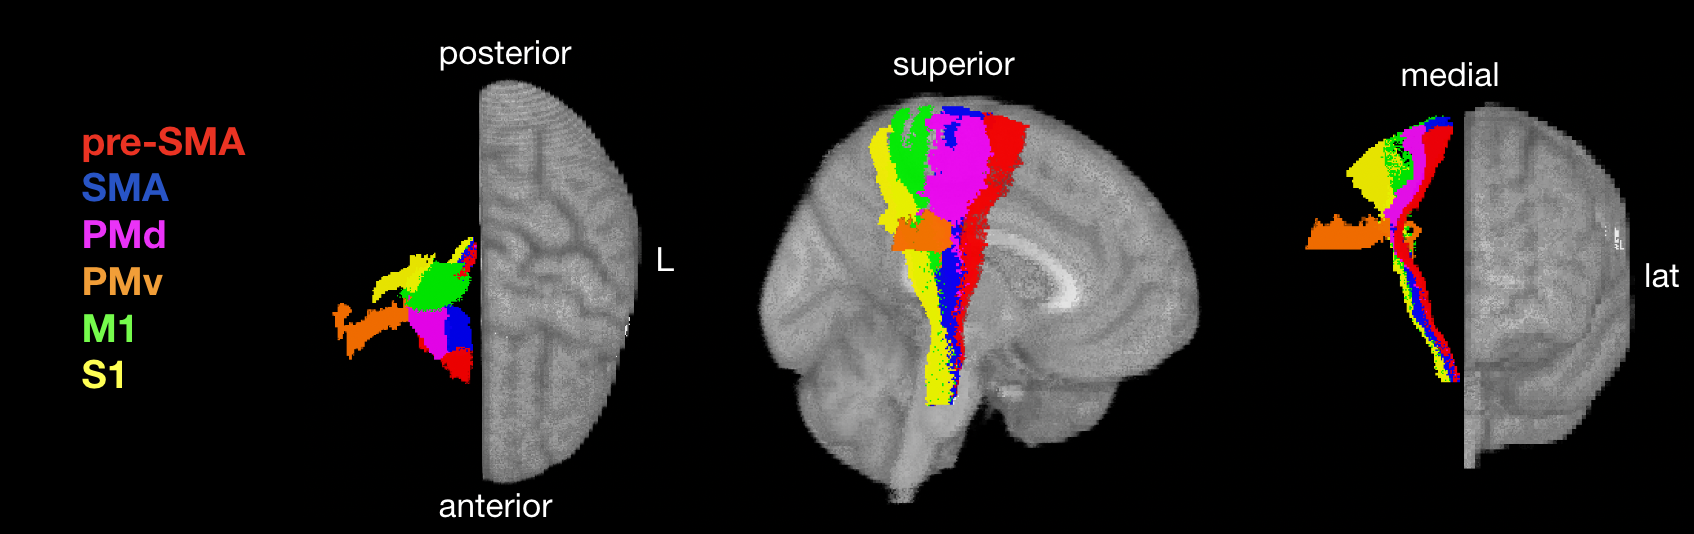
\includegraphics[width=1.0\linewidth]{figures/smatt_template.png}
\caption{Sensorimotor area tract template (right hemisphere visualized). Includes primary motor cortex (M1), dorsal premotor cortex (PMd), ventral premotor cortex (PMv), supplementary motor area (SMA), pre-supplementary motor area (pre-SMA), primary sensory cortex (S1).
}
\label{smatt_template}
\end{figure} 
\begin{figure}[]
\centering
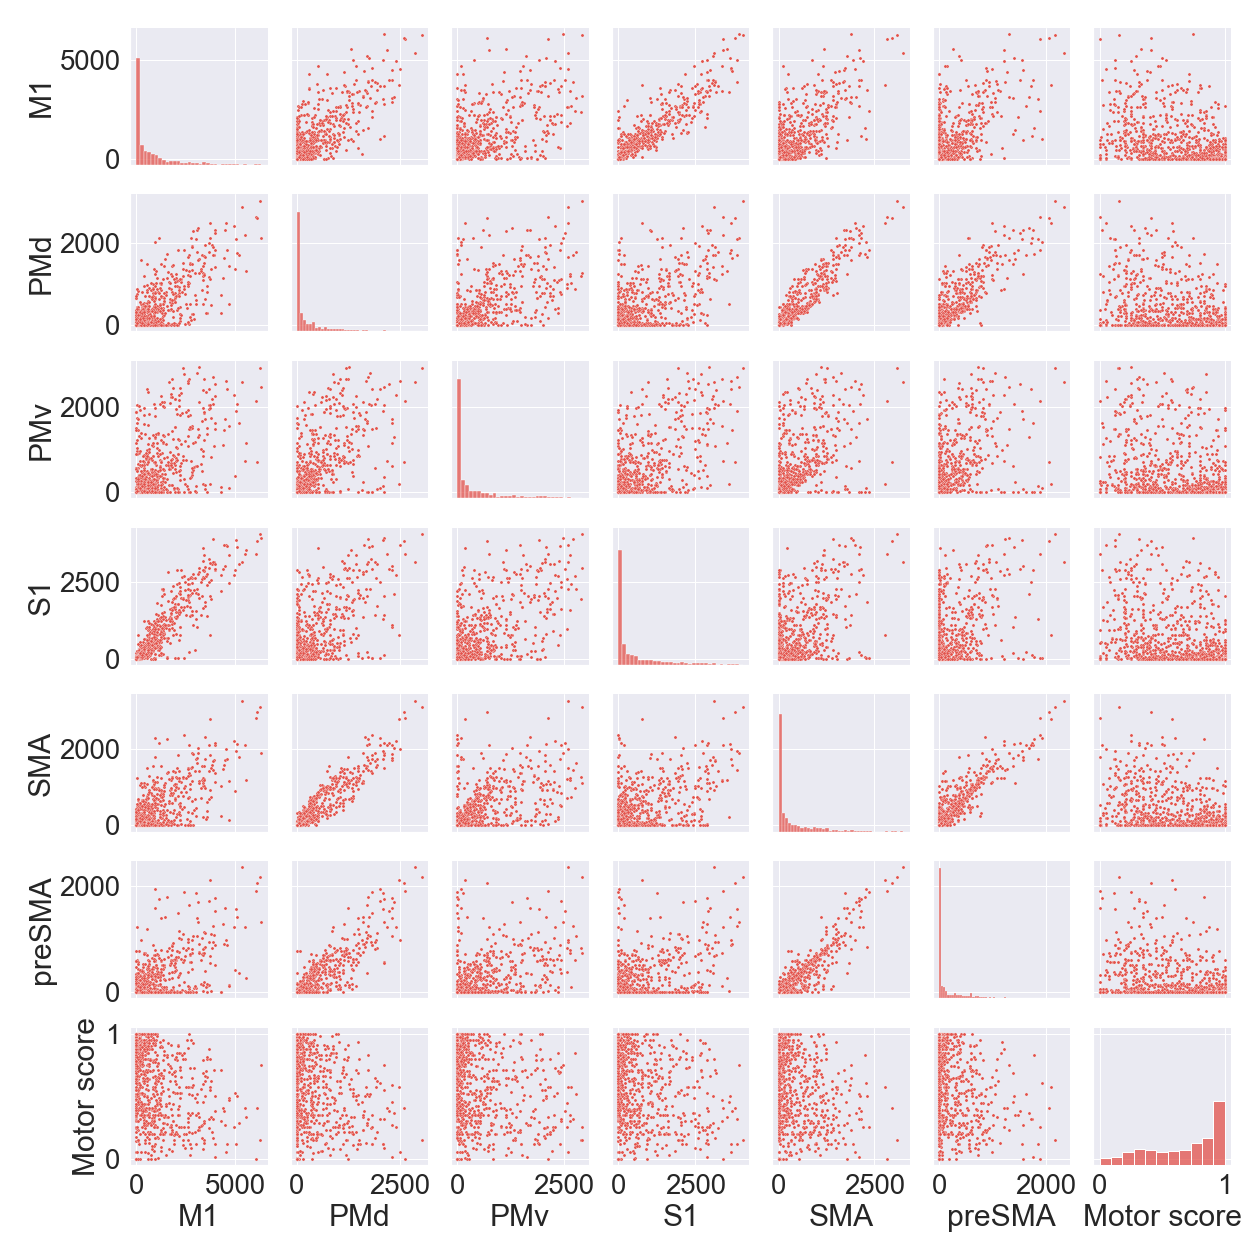
\includegraphics[width=0.8\linewidth]{figures/SMATT_scatterplts.png}
\caption{Correlations between lesion load calculated for each ipsilesional tract in the sensorimotor area tract template atlas.}
\label{smatt_pairwise_correlations}
\end{figure}


Previously, \cite{Ito2022-em} have shown that models that use the corticospinal tract lesion load fibers originating the ventral premotor cortex in addition to lesion load of the primary motor cortex have the strongest associations with motor scores.

Corticospinal tract segmentations were obtained from the sensorimotor area tract template (SMATT), a set of 6 tracts derived from probabilistic tractography seeded in primary motor cortex (M1), dorsal and ventral premotor cortex (PMd and PMv, respectively), supplementary motor area (SMA), pre-supplementary motor area (pre-SMA), and primary somatosensory cortex (S1) (Figure \ref{smatt_template}) (\cite{Archer2018-ti}).

Motor scores were predicted using regression models with these 6 features as inputs (as damage to all tracts is highly correlated, \cite{Ito2022-em}), (Figure (\ref{smatt_pairwise_correlations}).f

\subsubsection{Data-driven feature selection}
%\subsubsection*{Deriving ChaCo scores (change in connectivity) from lesion masks}

\begin{figure}[htp]
\centering
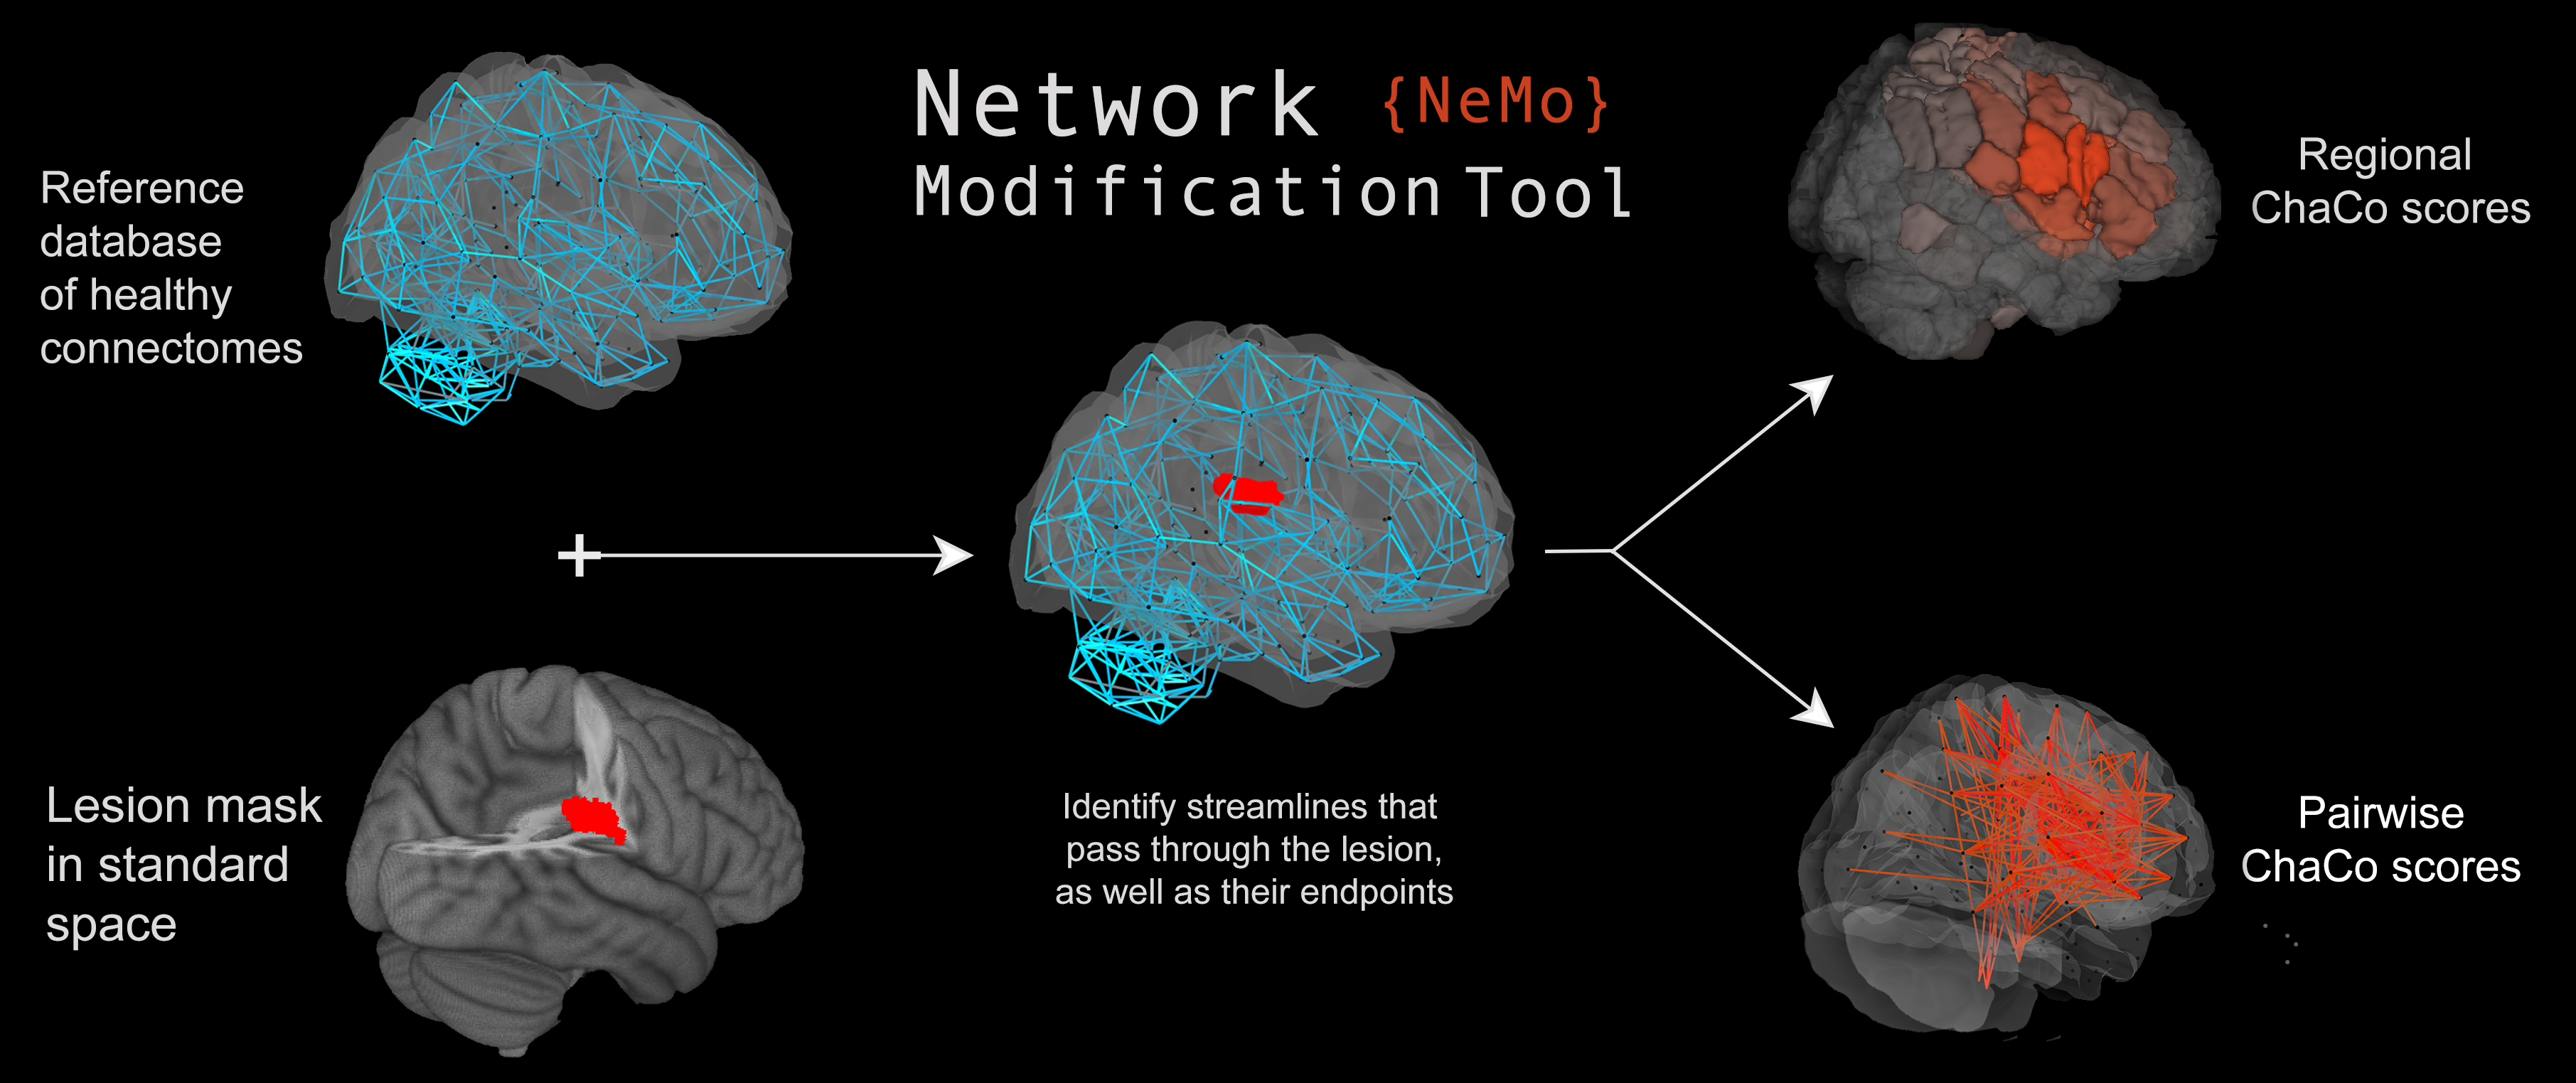
\includegraphics[width=1.0\linewidth]{figures/NetworkModificationTool.png}
\caption{Overview of the Network Modification tool. Binary lesion masks in MNI space representing the presence of a stroke lesion in a given voxel are provided by the user. Each lesion mask is embedded into 420 unrelated healthy structural connectomes (separately for each healthy subject) and the regional or pairwise change in connectivity (ChaCo) scores are calculated and averaged across healthy subjects. }
\label{nemotool}
\end{figure}
Lesion masks in $1mm^3$ MNI v6 space were processed with the Network Modification Tool v2 (NeMo) pipeline (\cite{Kuceyeski2013-nk}) (https://github.com/kjamison/nemo for more detailed information). Given a lesion mask, the NeMo tool produces outputs that reflect the impact of the lesion on the structural connectivity between gray matter regions. The NeMo tool identifies every white matter streamline that intersects with a lesion and determines the brain regions at the endpoints of those streamlines, whose structural connections we expect to be disrupted (Figure \ref{nemotool}). The NeMo tool uses a reference structural connectome (SC) dataset of 420 unrelated subjects from the Human Connectome Project Young Adult database. Structural connectivity for HCP subjects was obtained using deterministic tractography (SD stream) with dynamic seeding, with additional SIFT2 weighting for each of 5 million streamlines (\cite{Smith2015-eb}).


We extracted two outputs from the NeMo tool that reflect the impact of the lesion on connectivity between brain regions:

\begin{enumerate}
\item Regional change in connectivity (ChaCo) scores: the ratio of (disrupted streamlines)/(total streamlines) for each region.
\item Pairwise change in connectivity (ChaCo) score: the ratio of (disrupted streamlines)/(total streamlines) for each region-pair.
\end{enumerate}

In such a high-dimensional setting (i.e. using all possible structural connections or brain regions to predict outcomes, $n<<p$), it is necessary to employ a feature selection step to avoid overfitting. This was performed in a data-driven capacity; features were not chosen based on prior literature, because inference and prediction are different goals and the feature maps derived from both types of studies can vary widely (\cite{Sperber2021-lw, Bzdok2020-py}). We further employ ridge regression as a feature reduction step to account for multicollinearity of features. 

Ridge regression models were trained and evaluated using a 5-fold nested cross-validation loop. These multivariate models have been shown to produce good predictions of post-stroke impairment using imaging data due to their ability to capture multivariate patterns of stroke damage (\cite{Salvalaggio2020-pe} and account for multicollinearity in the data). In the outer loop, the data was split into training and test partitions. Training data was further partitioned into training and validation in the inner loop. In the inner loop, two hyperparameters were optimized: the amount of regularization on regression coefficients ($\lambda$) and the number of features to include ($\kappa$) after a feature selection step. The $\kappa$ values searched for FS86 (3192 non-zero edges) spanned 30 values from $2^2$ to $2^{11.64}$ (3192) in base-2 logarithmic steps, for pairwise models, and spanned 100 values from 1 to 286, in linear steps of 3 for the regional models. The $\kappa$ values searched for shen268  (25057 non-zero edges) spanned 30 values from $2^2$ to $2^{14.6129}$ (25057). The regularization coefficient $\lambda$ was chosen via grid search between $\lambda = 10^{-2}$ and $10^2$ in base-10 logarithmic steps for FS86, and between $\lambda = 10^{-2}$ and $10^3$ in base-10 logarithmic steps for Shen-268. These $\lambda$ ranges were chosen based on visualizations of the grid search space using a randomly chosen partition of training data (Figure ?) to ensure that a global maximum was obtained.

\subsection{Feature selection}
Ridge regression models on the full-dimensional input were originally attempted. However, they did not converge, likely because the number of predictors far exceeds the number of subjects (i.e., $p >> N$). Therefore, the full set of non-zero edge weights (3655 for FS86 and 35778 for Shen-268, for pairwise models, and 86 for FS86 and 268 for Shen-268, for regional models) was reduced via. a feature selection step to limit the risk of overfitting (\cite{Calesella2021-kp}). In this step, the edge weights were correlated with cognitive test scores in the training data using Pearson's correlation coefficient, and the $\kappa$ most highly correlating edges (by absolute value) were retained in the model, where $\kappa$ was determined with cross-validation as described above. Importantly, this feature selection was performed after data was split into training and test sets, such that no hold-out test data is used in the selection of the set of feature weights (\cite{Hastie2001-or}). 

\subsection{Model performance}
The performance of the model was assessed by calculating the coefficient of determination, or $R^2$, which captures the percent of variation in cognitive scores explained by the variation in the model predictors. 




\begin{tabular}{|l|l|r|r|r|r|}
%\captionof{table}{Site-specific demographic data.}
\hline {} &  Site &   N. &  N. F &  Mean age &  Mean normed motor \\ \hline
\textbf{0 } &  r001 &  39 &         10 &     59.62 &               0.62 \\ 
\textbf{1 } &  r002 &  12 &          6 &     65.75 &               0.45 \\
\textbf{2 } &  r003 &  15 &          6 &     59.53 &               0.26 \\ 
\textbf{3 } &  r004 &  19 &          7 &     44.63 &               0.20 \\ 
\textbf{4 } &  r005 &  27 &         12 &     64.93 &               0.67 \\
\textbf{5 } &  r009 &  57 &         16 &     67.84 &               0.92 \\ 
\textbf{6 } &  r010 &  26 &          7 &     57.15 &               0.97 \\ 
\textbf{7 } &  r011 &  28 &         10 &     57.21 &               0.89 \\ 
\textbf{8 } &  r015 &  15 &          0 &     59.60 &               0.72 \\ 
\textbf{9 } &  r017 &  14 &          0 &     57.43 &               0.52 \\
\textbf{10} &  r018 &  11 &          0 &     59.73 &               0.71 \\ 
\textbf{11} &  r021 &  12 &          0 &     60.83 &               0.90 \\
\textbf{12} &  r022 &  14 &          0 &     57.86 &               0.57 \\ 
\textbf{13} &  r023 &  14 &          8 &     58.00 &               0.43 \\ 
\textbf{14} &  r024 &  21 &          0 &     61.43 &               0.90 \\ 
\textbf{15} &  r025 &  16 &          3 &     64.19 &               0.73 \\ 
\textbf{16} &  r027 &  28 &          8 &     58.18 &               0.31 \\
\textbf{17} &  r028 &  21 &          6 &     58.14 &               0.74 \\
\textbf{18} &  r029 &   5 &          0 &     61.20 &               0.71 \\ 
\textbf{19} &  r031 &   1 &          0 &     52.00 &               0.68 \\ 
\textbf{20} &  r033 &   5 &          0 &     50.00 &               0.62 \\ 
\textbf{21} &  r034 &  15 &          6 &     57.26 &               0.80 \\ 
\textbf{22} &  r035 &  15 &          6 &     62.20 &               0.63 \\ 
\textbf{23} &  r038 &  18 &          7 &     62.17 &               0.88 \\ 
\textbf{24} &  r040 &  14 &          7 &     60.64 &               0.65 \\ 
\textbf{25} &  r042 &  22 &         11 &     50.55 &               0.61 \\ 
\textbf{26} &  r044 &   4 &          0 &     69.25 &               0.52 \\ 
\textbf{27} &  r045 &   4 &          1 &     59.75 &               0.48 \\ 
\textbf{28} &  r046 &  12 &          4 &     60.00 &               0.47 \\ 
\textbf{29} &  r047 &  44 &         14 &     64.84 &               0.62 \\
\textbf{30} &  r048 &  43 &         16 &     65.88 &               0.66 \\ 
\textbf{31} &  r052 &  32 &         12 &     61.09 &               0.41 \\ 
\textbf{32} &  r053 &   2 &          1 &     65.00 &               0.63 \\ 
\hline
\end{tabular}





\subsubsection*{Code availability}

\section{Results}



\begin{figure}
\begin{subfigure}{1\textwidth}
  \centering
  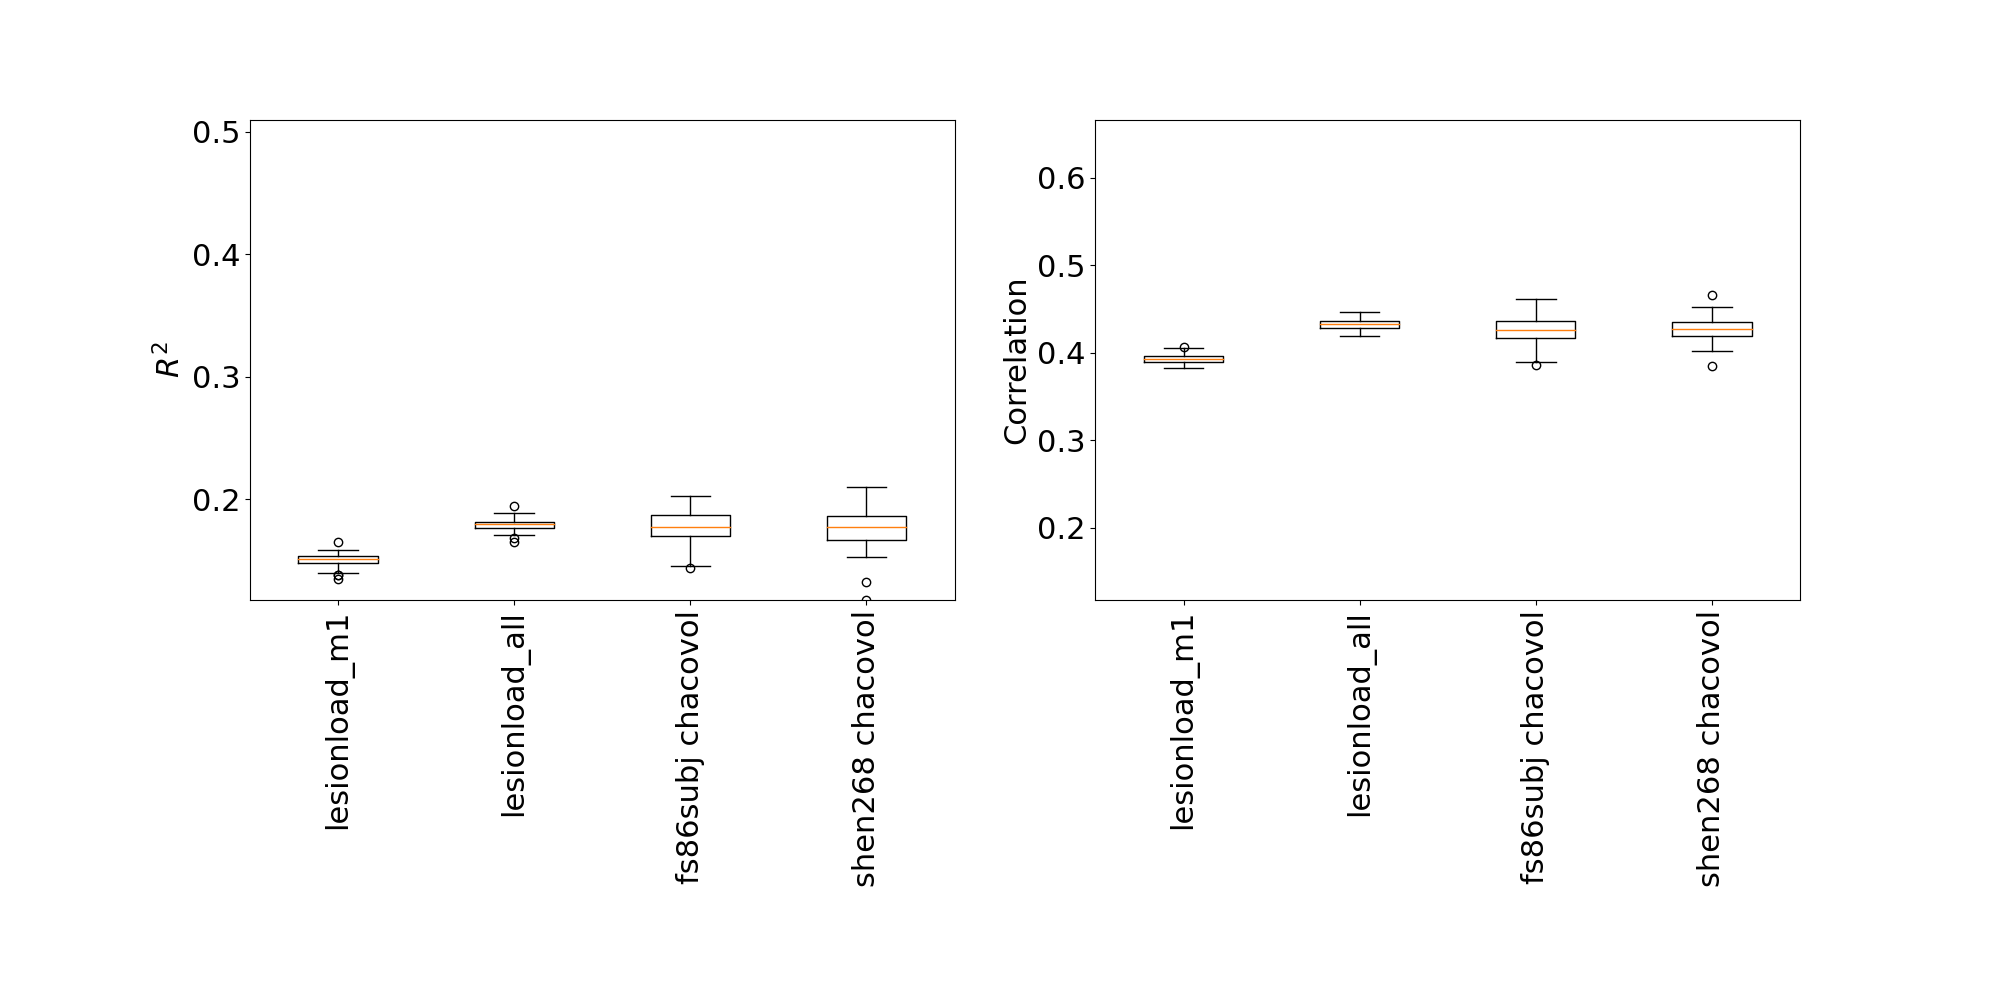
\includegraphics[width=1\linewidth]{figures/boxplots_1.png}
  \caption{Analysis 1}
  \label{fig:sfig1}
\end{subfigure}
\begin{subfigure}{1\textwidth}
  \centering
  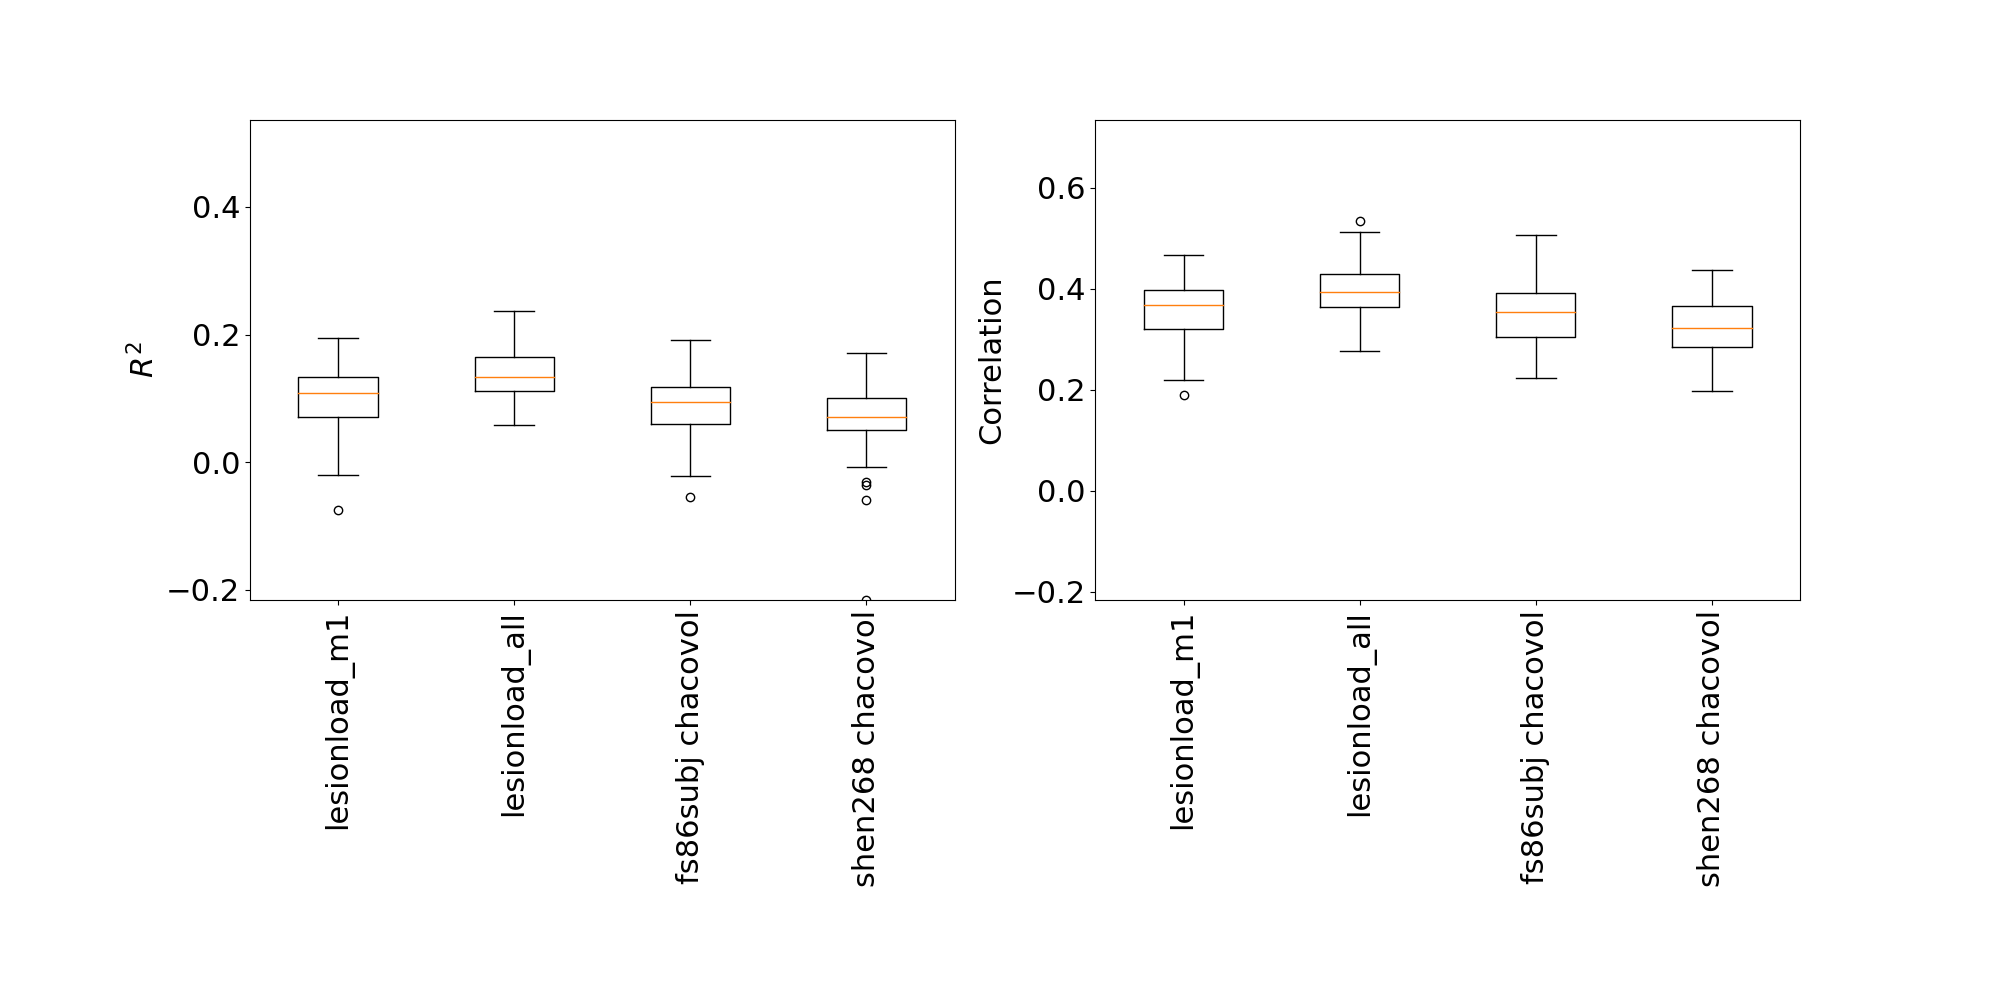
\includegraphics[width=1\linewidth]{figures/boxplots_2.png}
  \caption{Analysis 2}
  \label{fig:sfig1}
\end{subfigure}
\begin{subfigure}{1\textwidth}
  \centering
  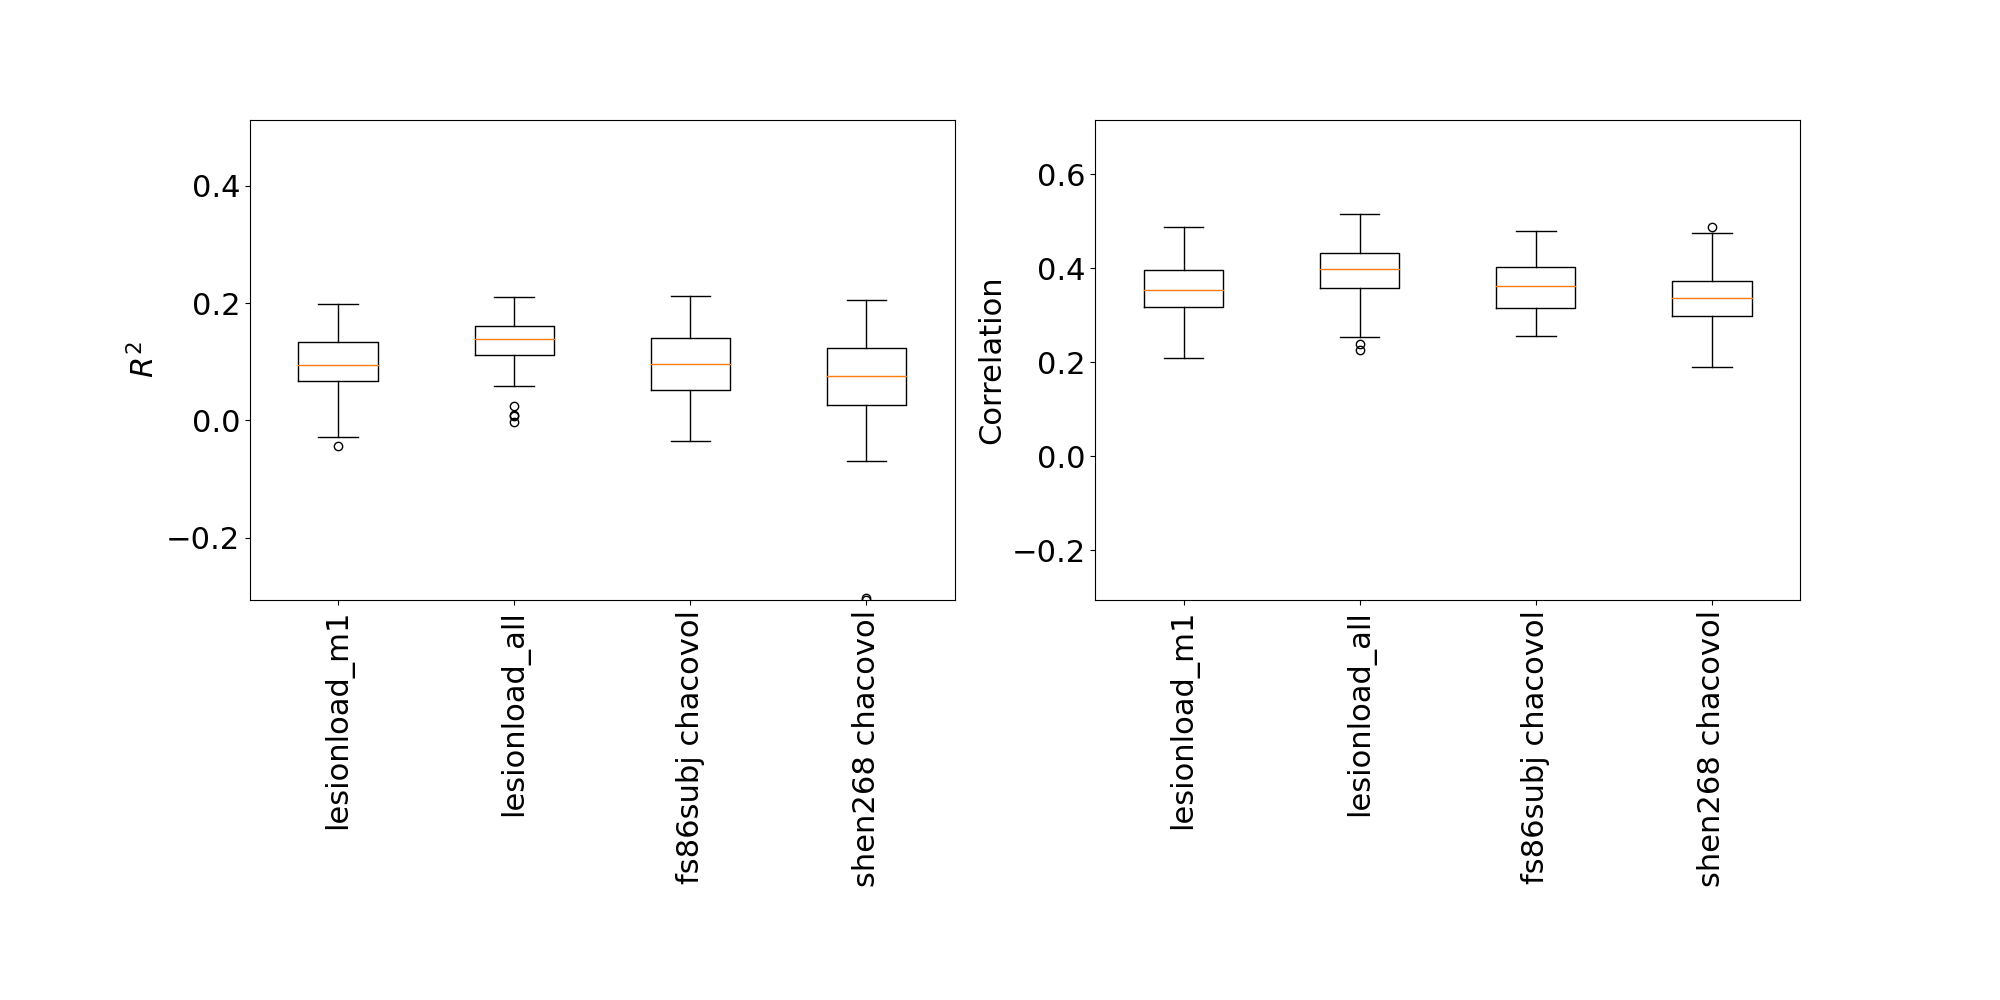
\includegraphics[width=1\linewidth]{figures/boxplots_3.png}
  \caption{Analysis 3}
  \label{fig:sfig1}
\end{subfigure}
\caption{Results from models.}
\label{fig:fig}
\end{figure}




\begin{figure}[htp]
\centering
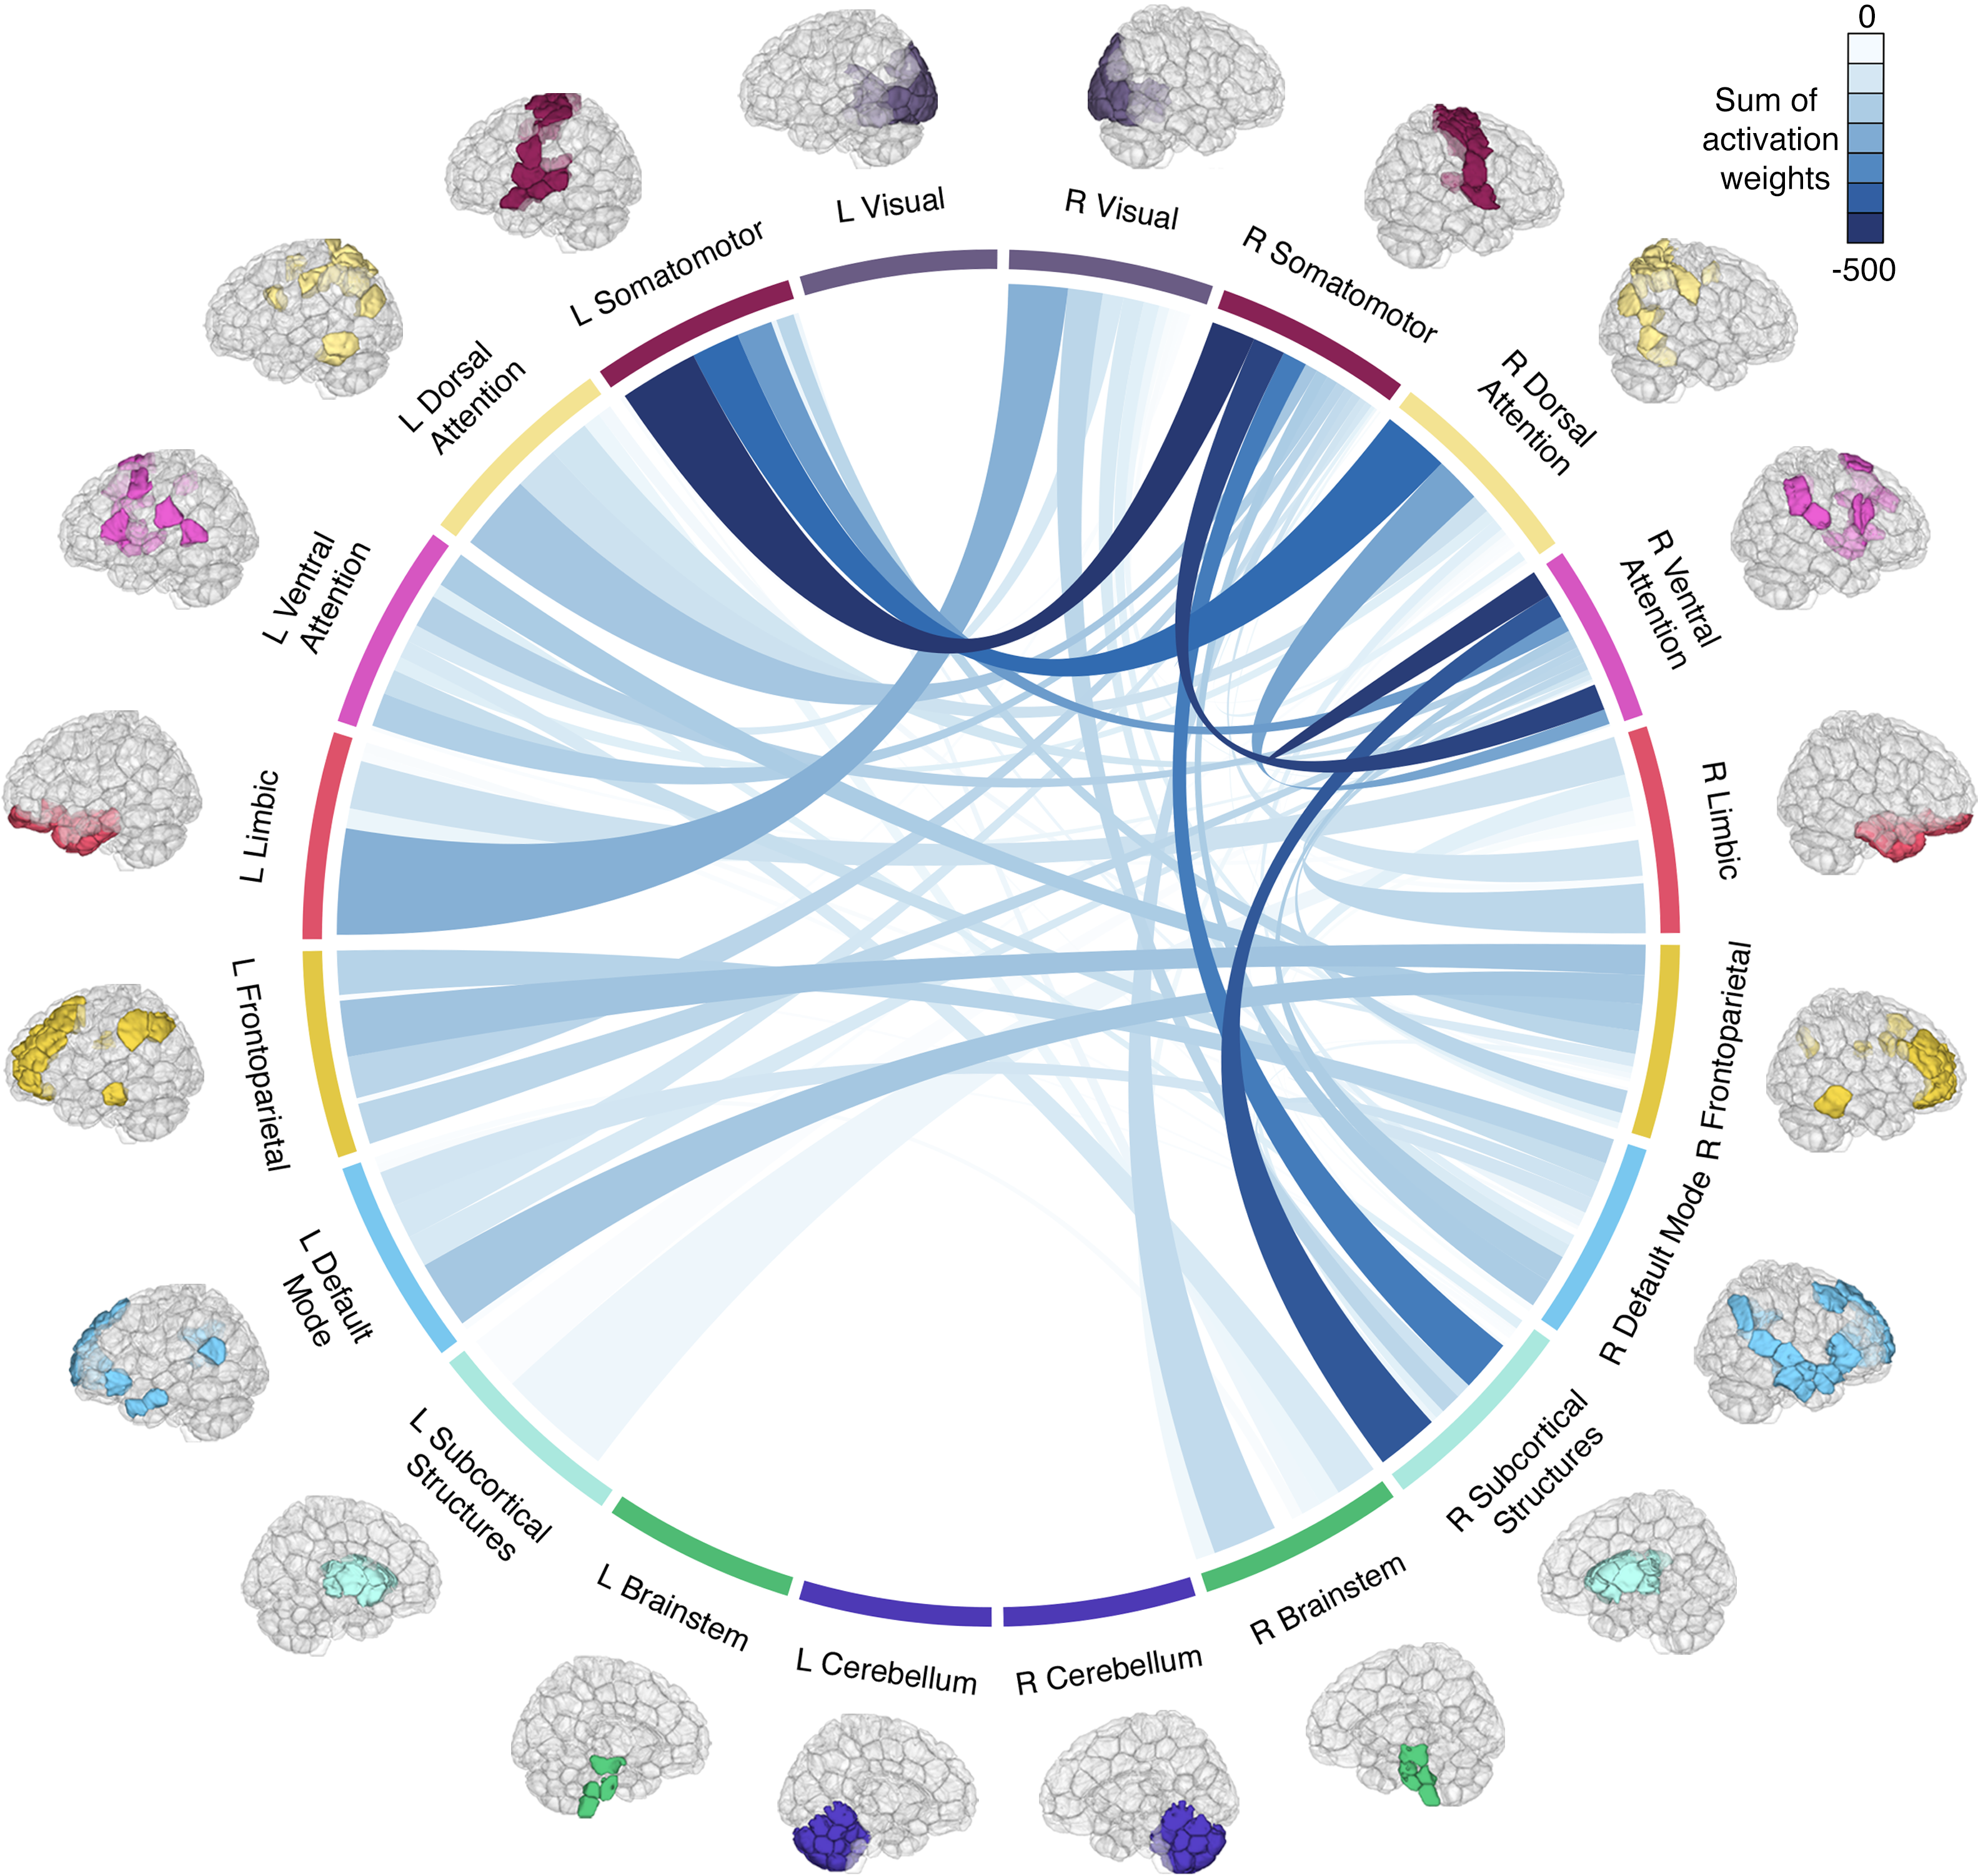
\includegraphics[width=1.0\linewidth]{chorddiagram_stdCV_LRsplit_onebrain.png}
\caption{Activation Weights.}

\label{}

\subsection{Cortical atrophy}

\end{figure}

\section{Discussion}

\subsection*{Predicting chronic motor scores from structural disconnection: CST lesion load}
In \cite{Pineiro2000-dv} original CST mask paper; looked at cross sectional area of CST occupied by stroke and related it to motor score at 1 month, $r^2 = 0.82$.

In \cite{Jang2008-ns} pontine infarct subjects (25) with CST damage (from DTI) in acute stage have worse chronic motor scores. 

In \cite{Zhu2010-qh}, CST-ll observed at chronic stage is predictor of chronic stroke motor impairment in moderate to severe stroke, not lesion size per se. Regression analyses with $R^2 = 0.72$ for weighted lesion load, 50 patients. Weighted lesion load is accounting for the narrowing of the CST as it descends; slicewise adjustment. 

Similarly in \cite{Lindenberg2010-pa}, descending white matter tract damage (anterior and posterior descending primary motor pathways, not just PT) predicts chronic outcome.

In \cite{Lam2018-xh}, they assess the ability of the CST lesion load to predict chronic CMSA-motor and ARAT scores. CST ll accounted for 23$\%$ and 24$\%$ of the variance in motor scores, in 27 subjects with upper limb impairments.

In \cite{Feng2015-du} wCST-LL is a good predictor of 3 month FM outcome in subjects with severe initial injury ($R^2 = 0.47$).

In \cite{Lin2019-hy}, CST injury taken from acute imaging explained ~20 percent of the variance in the magnitude of REALIZED upper extremity recovery (i.e. recovery adjusted for the different extents of recovery based on initial impairment) at the chronic stage.

In \cite{Ito2022-em}, CST-ll is calculated separately for descending tracts from M1, S1, SMA, preSMA, PMv, and PMd; roughly 50 percent of CST descending fibers are from premotor areas. Use SMATT toolbox. PMv and M1 classify FM severity groups better than M1 alone; PMv has less collinearity with other tracts.

In \cite{Hayward2022-hv}, WM microstructure of the CC (FA) relates to motor impairment in severe and mild/moderate. 

\subsection*{Predicting chronic motor scores from structural disconnection: alternative measures}
In \cite{Dulyan2021-jf}, they predict 3 month and 1 year motor outcomes for L and R deficits separately by using disconnectome components. Show a median/mode R of 0.56 and 0.5 for 3 months and 1 year prediction respectively (with permutations). If we're just going to square the R values and call that explained variance, they get 31 percent explained variance for 1 year post stroke left motor deficits, and 4 percent explained variance for 1 year post stroke right motor deficits. The methods of this preprint are questionable, but they do evaluate their model on held-out data.

In \cite{Peters2018-tf}, argue that Wallerian degeneration (WD) which is detected as early as 2 weeks post stroke, produces changes to cortex beyond the lesion site and may be predictive of chronic motor impairments. CST fibers originate from the premotor and primary motor areas. Subcortical areas like the thalamus and red nucleus are also implicated in movement. Cortico-subcortical connectivity may be related to motor behaviour. Looked at lesion overlap with cortical and subcortical areas. Also did DTI tracking to get connectivity strength between M1, PMC, SMA. SC between ipsilesional M1/SMA and thalamus related to motor scores.  

In \cite{Salvalaggio2020-pe} voxelwise SDC, then PCA and ridge regression and LOOCV. Predictions of motor scores 2 weeks post-stroke from SDC give an $R^2 = 0.37$.

In Rondina et al., 2017...
In \cite{Rondina2016-ds} they show that theory-driven feature selection, including areas from the premotor/frontal areas, better predicts motor outcome than just looking at CST-related features. Voxels (lesion voxels) associated with chronic motor performance (via mass univariate voxel GLMs) not found in CST but in pre and post central gyrus.

In \cite{Sperber2021-lw} and \cite{Bzdok2020-py} they discuss the difference between inference and prediction.  \cite{Sperber2021-lw} demonstrate that the areas that may be useful for prediction of motor deficits after stroke may not be clinically meaningful. Related to \cite{Mah2014-cb}, showing how patterns of damage from lesion-symptom mapping are biased/shifted due to vasculature.

\clearpage

\newcommand{\beginsupplement}{%
\setcounter{table}{0}
\renewcommand{\thetable}{S\arabic{table}}%
\setcounter{figure}{0}
\renewcommand{\thefigure}{S\arabic{figure}}%
}

\printbibliography

\beginsupplement
\section*{Supplementary Figures}

\end{document}